%  !TeX  root  =  user_guide.tex

\chapter{Lavorare con i dati raster}\label{label_raster}
\index{layer raster}

% when the revision of a section has been finalized, 
% comment out the following line:
%\updatedisclaimer

Questa Sezione descrive come visualizzare ed impostare le proprietà dei dati
raster. 
\qg usa la libreria GDAL per l'accesso in lettura/scrittura a formati raster
\footnote{Il supporto ai raster GRASS è fornito da un plugin fornitore dati nativo di QGIS.}
tipo Arc/Info Binary Grid,\index{Arc/Info Binary Grid}
Arc/Info ASCII Grid,\index{Arc/Info ASCII Grid} GeoTIFF,\index{GeoTIFF}
Erdas Imagine\index{Erdas Img.} e molti altri. 

Alla data del presente documento, la libreria GDAL \cite{GDALweb} supporta più di 
100 formati raster. La lista completa è disponibile alla pagina web 
\url{http://www.gdal.org/formats_list.html}.

\textbf{Nota}: per varie ragioni, \qg potrebbe non gestire alcuni dei formati 
elencati nella pagina web citata. Ad esempio, alcuni formati richiedono la 
presenza di librerie commerciali di terze parti oppure l'installazione di 
GDAL è avvenuta senza il supporto al formato che si intende usare. Quando si 
carica un raster in \qg solo i formati ben testati appariranno nell'elenco 
dei tipi di file; altri formati non testati possono essere caricati 
selezionando *.*.

Per caricare e lavorare con dati raster di GRASS, fare riferimento alla Sezione~\ref{sec:grass}.

\section{Cosa sono i dati raster?}\label{label_whatsraster}
\index{layer raster!definizione}

I dati raster sono matrici di celle discrete che rappresentano elementi della 
superficie terrestre o dell'ambiente al di sopra o al di sotto di essa. 
Ogni cella nella matrice raster ha la stessa dimensione e le celle sono 
solitamente rettangolari (in \qg saranno sempre rettangolari). Esempi
tipici di dati raster sono quelli provenienti dal telerilevamento come le
fotografie aeree, le immagini da satellite e dati modellati come le matrici dell'elevazione.

I dati raster di solito non hanno associato un database contenente i dati 
descrittivi di ogni cella, diversamente dai dati vettoriali, e sono geocodificati 
in base alla risoluzione del pixel e alle coordinate x/y di un angolo del raster.

Per posizionare e visualizzare correttamente un raster, \qg legge le informazioni di 
georeferenziazione incorporate nel file del raster (ad es. GeoTiff) o gestite in un 
apposito file noto come "world file".\index{layer raster!georeferenziazione}
	
\section{Caricare dati raster in QGIS}\label{label_loadraster}

I layer raster possono essere caricati tramite lo strumento \toolbtntwo{mActionAddRasterLayer}{Aggiungi raster} 
o scegliendo la voce di menu \mainmenuopt{Layer} \arrow \dropmenuopttwo{mActionAddRasterLayer}{Aggiungi raster...}.
È possibile caricare più di un layer alla volta tenendo premuto il
tasto \keystroke{Ctrl} o \keystroke{Shift} e selezionando con il mouse 
più elementi nella finestra di dialogo \dialog{Apre
un raster supportato da GDAL}.\index{layer raster!caricamento}

Quando il layer è caricato è possibile cliccare sul suo nome nella legenda 
con il tasto destro del mouse per selezionare ed attivare opzioni specifiche o per
aprire la finestra per l'impostazione delle proprietà del layer raster.

\minisec{Menu contestuale per layer raster}

\begin{itemize}[label=--]
\item \dropmenuopt{Zoom all'estensione del layer}
\item \dropmenuopt{Zoom alla scala migliore (100\%)}
\item \dropmenuopt{Aggiungi alla panoramica}
\item \dropmenuopt{Rimuovi}
\item \dropmenuopt{Imposta il SR del layer}
\item \dropmenuopt{Imposta il SR del progetto dal layer}
\item \dropmenuopt{Proprietà}
\item \dropmenuopt{Rinomina}
\item \dropmenuopt{Aggiungi gruppo}
\item \dropmenuopt{Espandi tutto}
\item \dropmenuopt{Comprimi tutto}
\end{itemize}
	
\section{Proprietà raster}\label{label_rasterprop}

Per visualizzare ed impostare le proprietà di un layer raster, fare doppio
click sul nome del raster nella legenda o cliccare su di esso con il tasto
destro e scegliere \dropmenuopt{Proprietà} dal menu contestuale:\index{layer raster!menu contestuale}
La figura \ref{fig:raster_properties} mostra la finestra \dialog{Proprietà layer}. 
Ci sono diverse schede nella finestra: 

\begin{itemize}
 \item \tab{Stile}
 \item \tab{Trasparenza}
 \item \tab{Mappa colore}
 \item \tab{Generale}
 \item \tab{Metadata}
 \item \tab{Piramidi}
 \item \tab{Istogramma}
\end{itemize}

\begin{figure}[h]
  \begin{center}
   \caption{Finestra delle proprietà dei layer raster \nixcaption}\label{fig:raster_properties}\smallskip
   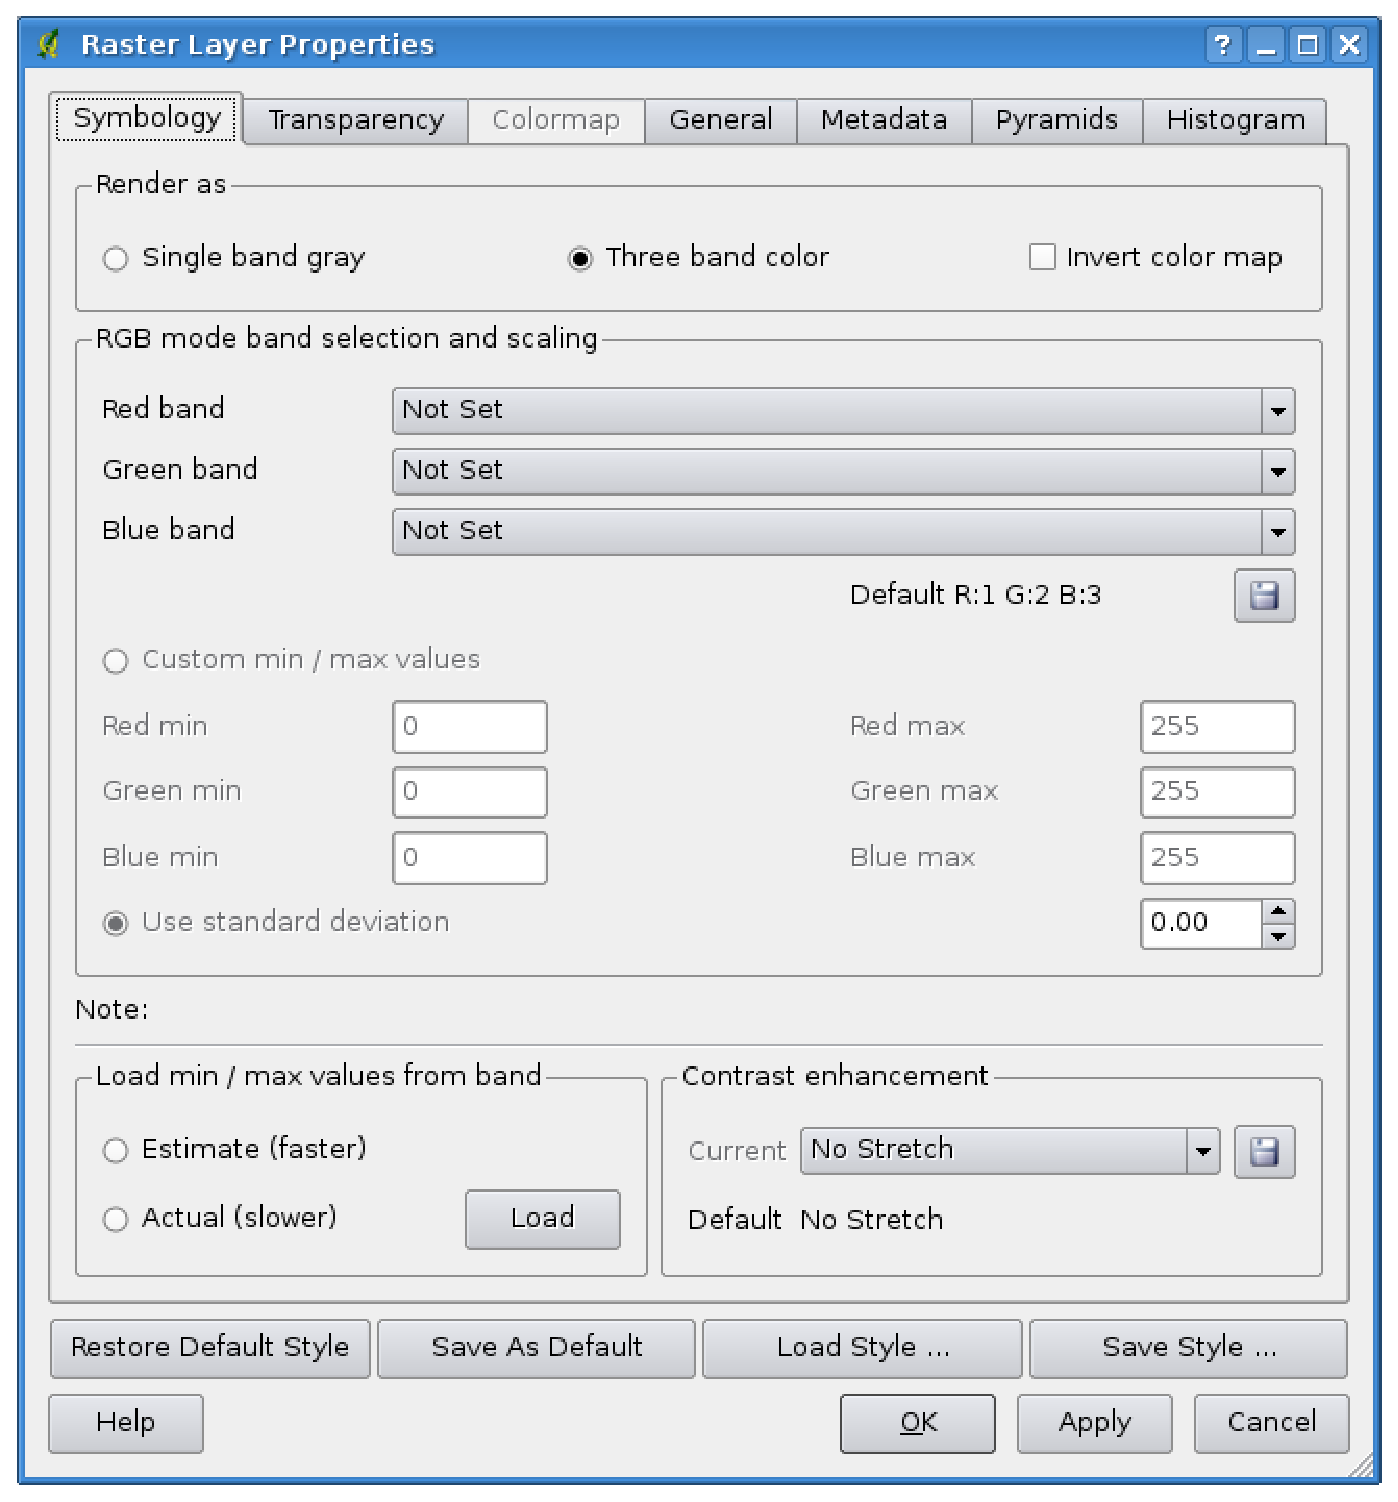
\includegraphics[clip=true, width=14cm]{rasterPropertiesDialog}
\end{center}  
\end{figure}

\subsection{Scheda Stile}\label{label_sombology}

QGIS può rendere a video i raster in due modi:\index{layer raster!canali supportati}

\begin{itemize}[label=--]
\item Banda singola grigia - una sola banda dell'immagine è resa in scala di grigi,
o in pseudo colore o ancora in freak out.
\item Tre bande di colore - tre bande dell'immagine, ognuna rappresentante la componente rosso o verde o blu, 
vengono composte per creare un'immagine a colori.
\end{itemize}

È possibile invertire i colori in modo che i quelli chiari diventino scuri e
viceversa selezionando la casella di controllo \checkbox{Inverti mappa colore}.

\minisec{Banda singola grigia}

Selezionando questa opzione vengono offerte due possibilità tra le quali
scegliere. Innanzitutto se il layer è multibanda è possibile scegliere quale
banda si desidera venga impiegata per la resa a video. 

La seconda opzione offre una selezione di mappe colore preimpostate per la
resa a video.

Le scelte possibili disponibili nel menu a tendina sono:
\selectstring{Mappa colore}{Scala di grigi}, impostazione di default.
Altre scelte possibili sono
\begin{itemize}
\item Pseudo colore
\item Freak Out
\item Mappa colore
\end{itemize}

Quando viene selezionata l'opzione \selectstring{Mappa colore}{Mappa colore},
la scheda \tab{Mappa colore} è abilitata. Si vedano ulteriori
informazioni al Capitolo \ref{label_colormaptab}.

QGIS restringe la visualizzazione dei dati per mostrare soltanto le celle i cui 
valori ricadono all'interno di una deviazione standard definita.\index{layer raster!deviazione standard} 
Ciò può essere utile quando nella griglia raster si hanno una o due celle 
con valori estremamente alti: questi hanno un impatto negativo sulla resa a video del raster.
Tale opzione è disponibile solo per immagini in pseudo colore o freak out. 

\minisec{Tra bande di colore}

Questa opzione offre un considerevole numero di possibilità di modifica
dell'aspetto del raster. Ad esempio è possibile cambiare il normale ordine RGB
delle bande e/o applicare una scala di colori in base ai valori min/max del
raster.

\begin{Tip}\caption{\textsc{Visualizzare una singola banda di un raster multibanda}}
Il modo corretto di visualizzare ad es. la sola banda rossa di
un'immagine multibanda non è quello di impostare le bande verde e blu a "Non
impostato", ma di impostare il tipo di immagine come scala di grigi e quindi
scegliere il rosso come banda da usare per il grigio.
\end{Tip} 

\subsection{Scheda Trasparenza} \label{rastertab:transparency}

\qg offre la possibilità di visualizzare ogni layer raster ad un diverso grado di trasparenza.\index{layer raster!trasparenza}
Per settare una \guiheading{Trasparenza globale}, impostare il cursore a scorrimento al livello di trasparenza desiderato
in maniera tale da consentire la visualizzazione degli eventuali layer sottostanti. 
L'uso di questa impostazione può essere molto utile nei casi in cui si
desideri sovrapporre ad es. ad una mappa delle ombreggiature del rilievo (shaded
relief-map) una mappa raster contenente delle classificazioni, così da dare  a quest'ultima un
aspetto tridimensionale.

La sezione \guiheading{Nessun valore} consente invece di definire la trasparenza per un certo valore del raster, 
che sarà quindi letto come un campo privo di dati del tipo {\em NODATA}. Di
conseguenza in corrispondenza di tutte le celle del raster contenenti quel
valore non verrà reso a video niente, determinando quindi una trasparenza per
il valore specificato.

È possibile definire la trasparenza in maniera ancora più dettagliata e
personalizzata nelle Sezione \guiheading{Opzioni di trasparenza
personalizzate}, nella quale è possibile impostare il grado di trasparenza di
ogni singola cella (o pixel).
Ad esempio se si volesse utilizzare quest'ultima sezione per evidenziare l'acqua 
del raster \filename{landcover.tif} con una trasparenza del 20\%, 
bisognerà seguire la seguente procedura:

\begin{enumerate}
 \item Caricare il raster \filename{landcover}
 \item Aprire la finestra di dialogo \dialog{Proprietà} facendo doppio click
 sul nome del layer nella legenda o cliccando su di esso con il tasto destro del mouse e
 scegliendo \dropmenuopt{Proprietà} dal menu contestuale
 \item Selezionare la scheda \tab{Trasparenza}
 \item \label{enum:add} Cliccare sul pulsante
 \toolbtntwo{mActionNewAttribute}{Aggiungi un valore manualmente}. Nella lista
 pixel apparirà una nuova riga
 \item \label{enum:transp} Inserire il valore del raster per il quale si
 desidera modificare la trasparenza (si supponga 0 per questo esempio) e si
 imposti la trasparenza al 20\%
 \item Cliccare sul pulsante \button{Apply} per visualizzare il risultato.
\end{enumerate}

È possibile ripetere i passaggi \ref{enum:add} e \ref{enum:transp} per
impostare ulteriori valori con una trasparenza personalizzata.

Impostare la trasparenza personalizzata è alquanto semplice, ma la 
procedura può risultare laboriosa specie se si hanno molti valori da
impostare. Per ovviare a tale complicazione, è possibile salvare la 
lista delle impostazioni di trasparenza cliccando sul pulsante \toolbtntwo{mActionFileSave}{Esporta su
file} per non ripetere la procedura. 
Il pulsante \toolbtntwo{mActionAddRasterLayer}{Importa da file}, infatti, 
carica il file salvato e applica le impostazioni al raster selezionato.

\subsection{Scheda Mappa colore} \label{label_colormaptab}

La scheda \tab{Mappa colore} viene abilitata solo quando si imposta la resa
a video del raster come "Banda singola grigia" nella scheda \tab{Stile} 
(Capitolo \ref{label_sombology}).

Sono disponibili tre modalità di interpolazione del colore:
\begin{itemize}
\item Discrete
\item Lineare
\item Esatto
\end{itemize}

Il pulsante \button{Aggiungi elemento} aggiunge un colore alla tabella dei colori sottostante.
\button{Cancella elemento} elimina un colore dalla tabella dei colori.
\button{Ordina} ordina la tabella dei colori in funzione dei valori dei pixel della colonna Valore.  
Facendo doppio click su un valore della colonna Valore è possibile specificare o modificare il valore stesso.
Facendo doppio click sulla casella colorata a fianco del valore editato (colonna "colore) appare
la finestra di dialogo \dialog{Select color}, che permette di selezionare il colore da applicare 
a tutte le celle raster (o pixel) il cui valore corrisponde a quello appena editato.

In alternativa è possibile cliccare sul pulsante
\toolbtntwo{mActionNewAttribute}{Carica mappa colore dalla banda}, con il
quale viene caricata, se viene trovata o se disponibile, la tabella dei colori dalla banda.

La sezione \guiheading{Genera nuova mappa colore} consente di creare nuove
mappe colore per categoria. È sufficiente impostare il \selectnumber{Numero di elementi}{15} e cliccare poi su
\button{Classifica}. Attualmente è supportato il solo \selectstring{Modo di classificazione}{Equal Interval}\index{layer raster!classificazione}.

\subsection{Scheda Generale}\label{label_generaltab}

La scheda \tab{Generale} visualizza le informazioni di base sui raster selezionati,
incluso il percorso alla sorgente dati e il nome (modificabile a
piacere) visualizzato in legenda. Viene inoltre mostrata una miniatura del layer, 
la legenda dei simboli e la gamma di colori. \index{layer raster!proprietà}

È qui possibile attivare la funzione che setta la visibilità del layer
in base alla scala della mappa, attivando l'apposita casella di controllo ed
impostando l'intervallo di scale entro il quale si vuole che il layer venga
reso a video.

Viene inoltre fornita l'indicazione del sistema di riferimento spaziale (SR)
impostato per il layer raster in formato stringa PROJ.4. Il SR è modificabile
cliccando sul pulsante \button{Cambia}.

\subsection{Scheda Metadati}\label{label_metatab}

La scheda \tab{Metadati} mostra una serie di informazioni sul layer
raster, come ad es. le statistiche riguardanti ogni banda. Le statistiche sono
disponibili in questa scheda solo dopo averle raccolte cliccando nella
scheda \tab{Istogramma} sul pulsante \button{Aggiorna} in basso a destra 
(Capitolo \ref{label_histogram}.

Si tratta quindi di una scheda meramente informativa nella quale non è
possibile modificare alcun valore.

\subsection{Scheda Piramidi}\label{raster_pyramids}

I layer raster ad alta risoluzione possono rallentare notevolmente
l'esplorazione della mappa in QGIS. Creando copie a bassa risoluzione dei dati 
(piramidi) le prestazioni possono venire incrementate notevolmente in quanto 
QGIS sceglierà la risoluzione migliore in funzione del fattore di zoom.
\index{layer raster!piramidi}
\index{layer raster!risoluzione piramidi}

Per creare piramidi è necessario avere i permessi in scrittura nella cartella 
contenente il dato originale: in questa cartella verranno salvate le copie a 
bassa risoluzione. \\
Sono disponibili i seguenti metodi di ricampionamento:
\begin{itemize}
\item Media
\item Vicino più prossimo (metodo Nearest Neighbour)
\end{itemize}

Quando viene attivata la casella di controllo \checkbox{Crea piramidi interne
se possibile} QGIS crea e memorizza le piramidi direttamente nel file raster, 
invece di copie multiple separate.

Si evidenzia che la costruzione delle piramidi può alterare il dato originale
in maniera irreversibile, quindi si raccomanda di fare una copia di backup del
raster di partenza prima di eseguire l'operazione.

\subsection{Scheda Istogramma}\label{label_histogram}

La scheda \tab{Istogramma} consente di visualizzare la distribuzione
\index{layer raster!istogramma} delle bande di colore nel layer raster.
Tali statistiche sono generate automaticamente nel momento in cui si accede 
alla scheda \tab{Istogramma}. 
È possibile selezionare quale banda mostrare nel diagramma selezionandola 
nella lista sulla sinistra della scheda. 

\begin{Tip}\caption{\textsc{Acquisire le statistiche del raster}}
Per ottenere le statistiche di un layer, impostarne la
rappresentazione in pseudocolore e cliccare su \button{Applica}. L'operazione
può richiedere molto tempo in funzione della quantità di dati contenuti nel
raster, delle impostazioni di analisi settate e delle capacità di calcolo
della macchina usata, attendere quindi pazientemente
che QGIS termini tale analisi.\index{layer raster!statistiche}
\end{Tip}

\section{Calcolatore raster}\label{sec:raster_calc}
\index{Raster!calcolatore raster}
\index{Calcolatore raster}

La finestra di dialogo \dialog{Calcolatore raster} del menu \mainmenuopt{Raster} 
permette di effettuare calcoli sulla base dei valori dei pixel di raster esistenti.
Il risultato viene salvato in un nuovo layer raster in uno dei formati supportati da GDAL. 

\begin{figure}[ht]
  \centering
    \includegraphics[clip=true, width=11.5cm]{raster_calculator}
    \caption{Calcolatore raster \nixcaption}\label{fig:raster_calculator}
\end{figure}

La sezione \textbf{Bande raster} elenca i layer raster caricati in QGIS.
Per aggiungere un raster nella casella Espressione del calcolatore raster, 
fare doppio click sul suo nome in Bande raster. 
Si possono usare gli operatori per costruire un'espressione o scriverla
direttamente nella casella delle espressioni.

Nella sezione \textbf{Layer di risultato} va definito il nome del raster risultato, 
l'estensione dell'area di calcolo che ne determinerà la risoluzione e il formato: se il layer in 
input ha una risoluzione diversa, i valori saranno ricampionati con l'algoritmo del 
vicino più prossimo.  

La sezione \textbf{Operatori} elenca gli operatori disponibili. Per aggiungere un operatore alla casella 
Espressione del calcolatore raster, cliccare sull'icona ad esso relativa. Sono disponibili 
operazioni matematiche (+ , - , * \dots), funzioni trigonometriche (sin, cos, tan, \dots), operatori 
logici (AND, OR).

Selezionando la casella di controllo \checkbox{Aggiungi al progetto}, il layer risultato sarà
aggiunto alla legenda e potrà essere visualizzato nella vista mappa.

\section{Analisi raster}\label{sec:raster_analysis}
\index{Raster!analisi raster}
\index{Analisi raster}

Oltre la calcolatore raster, ulteriori funzionalità di analisi raster sono fornite dal plugin GDALTools.
Si veda la sezione \ref{label_plugingdaltools} per le informazioni di dettaglio.

\FloatBarrier